\section{Instalacja Cygwin'a}
\begin{enumerate}
\item pobieramy najnowszą wersję Cygwin'a ze strony \verb|http://www.cygwin.com/setup.exe|
\item podczas instalacji wybieramy kolejno (po każdym klikając \verb|dalej|):
  \begin{itemize}
  \item ,,Install from Internet''
  \item podajemy katalog do instalacji, np. \verb|C:\cygwin|
  \item podajemy miejsce, gdzie mają trafiać ściągane pliki, np. \verb|C:\cyg_install|; po instalacji, można je usunąć
  \item jeśli łączymy się przez proxy, ustawiamy je w tym kroku, w przeciwnym wypadku - ,,Direct Connection''
  \item jako stronę, z której będą pobierane dane, możemy wybrać dowolną (wracamy i wybieramy inną, gdyby któraś z nich nie działała)
  \item w tym kroku rozwijamy listę ,,Net'' i wybieramy z niej ,,rsync'' - klikamy na \verb|Skip|, aż pojawi się najnowsza wersja (patrz rys. \ref{cyg_inst}); można tu skorzystać także z wyszukiwarki
  \item jeżeli chcemy korzystać z szyfrowanego połączenia poprzez SSH, wybieramy pakiet \verb|openssh|, także z listy ,,Net''
  \item na zakończenie instalacji możemy ustawić sobie skróty na pulpicie i/lub w Menu Start
  \end{itemize}
\end{enumerate}
W katalogu \verb|C:\cygwin\bin| pojawia nam się pożądana aplikacja \verb|rsync.exe|.
\begin{figure}[h!]
	\centering
	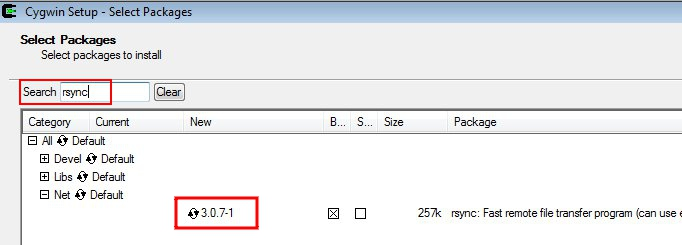
\includegraphics[width=0.8\textwidth]{../img/i4.jpeg}
	\caption{Instalacja rsync w Cygwin'ie}
	\label{cyg_inst}
\end{figure}

\newpage
\section{Skrypty}
\begin{enumerate}
\item \textbf{uruchamiamy dowolny edytor tekstowy, np. Notatnik} (rys. \ref{cmd})
\begin{figure}[h!]
	\centering
	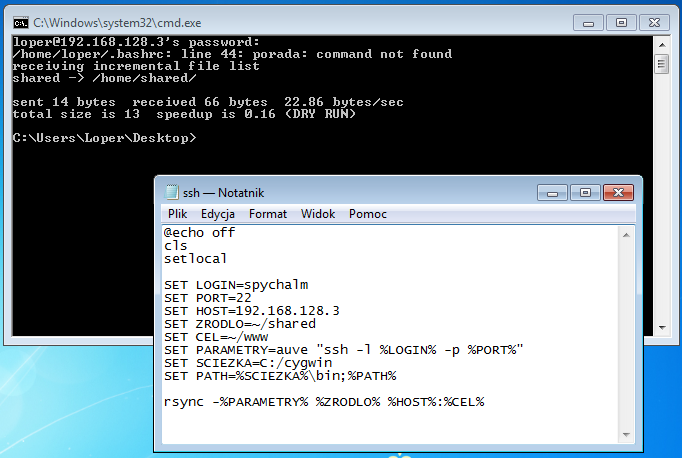
\includegraphics[width=0.6\textwidth]{../img/cmd.jpg}
	\caption{Okno notatnika i wiersza poleceń}
	\label{cmd}
\end{figure}
\item \textbf{kopiujemy i wklejamy wybrany skrypt z poniższych:}
\subsection*{synchronizacja zdalna:}
\begin{verbatim}
@echo off
cls
setlocal

SET HOST=
SET PARAMETRY=
SET CEL=
SET ZRODLO=

SET SCIEZKA=C:\cygwin
SET PATH=%SCIEZKA%\bin;%PATH%
\end{verbatim}

\textbf{dopisujemy:}

(dla wysyłania)
\verb|rsync -%PARAMETRY% %ZRODLO% %HOST%:%CEL%|

(dla odbierania)
\verb|rsync -%PARAMETRY% %HOST%:%ZRODLO% %CEL%|

\subsection*{synchronizacja za pomocą SSH:}
\begin{verbatim}
@echo off
cls
setlocal

SET LOGIN=
SET PORT=

SET HOST=
SET PARAMETRY=
SET CEL=
SET ZRODLO=

SET SCIEZKA=C:\cygwin
SET PATH=%SCIEZKA%\bin;%PATH%
\end{verbatim}
\textbf{dopisujemy:}

(dla wysyłania) 

\verb|rsync -%PARAMETRY% -e "ssh -l %LOGIN% -p %PORT%" %ZRODLO% %HOST%:%CEL%|

(dla odbierania) 

\verb|rsync -%PARAMETRY% -e "ssh -l %LOGIN% -p %PORT%" %HOST%:%ZRODLO% %CEL%|

\item \textbf{ustawiamy zmienne}

\textbf{dla SSH:}
\begin{itemize}
\item \verb|SET LOGIN=...| - login na koncie SSH,
\item \verb|SET PORT=...| - port SSH
\end{itemize}

\textbf{dla SSH i zdalnej:}
\begin{itemize}
\item \verb|SET HOST...| - adres lub nr IP serwera, na który wysyłamy/odbieramy dane
\item \verb|SET PARAMETRY=...| - parametry synchronizacji:
\begin{center}
\begin{tabular}{ r l }
-a & - tryb archiwalny (odpowiadający ,,-rlptgoD'') \\
-v & - bardziej szczegółowe informacje \\
-r & - rekursywnie wszystkie katalogi \\ 
-l & - zachowanie dowiązań symbolicznych \\
-u & - pomiń, jeśli nowsze u odbiorcy \\
-p & - zachowaj prawa dostępu \\
-t & - zachowaj czasy modyfikacji \\
-o & - zachowaj właściciela \\
-g & - zachowaj grupę \\
-e & - deklaruje powłokę do użycia \\
-z & - kompresuj dane podczas kopiowania \\
-n & - test działania (bez wprowadzania zmian) \\
-h & - liczby w czytelnej formie \\
-P & - pokaż pasek postępu \\
-D & - zachowaj potoki i nazwane gniazda\\
-L & - kopiuje pliki, na które wskazują dowiązania, zamiast nich \\
-q & - nie wypisuj błędów
\end{tabular}
\end{center}
\item \verb|SET CEL=...| - podajemy miejsce docelowe,
\item \verb|SET ZRODLO=...| - podajemy lokalizację źródłową; tutaj wymagane jest dłuższe wyjaśnienie.\\W Windowsie ścieżki składają się z litery dysku (np. C, D, E), dwukropka i odwróconego ukośnika (np. \verb|C:\katalog|). Użycie znaku dwukropka, w składni polecenia \verb|rsync|, zostałoby potraktowane jako ścieżka do katalogu zdalnego, dlatego stosujemy tu konwencję znaną z UNIX'a, to jest: zamieniamy odwrócone ukośniki na nieodwrócone, a w miejsce litery dysku wpisujemy \verb|/cygdrive/<litera_dysku>|. W ten sposób nasza przykładowa lokalizacja wygląda następująco: \verb|/cygdrive/c/katalog|.
\end{itemize}

\item \textbf{zapisujemy z rozszerzeniem ,,.bat'', np. ,,C:/skrypty/synchronizacja.bat''}

\item \textbf{uruchamiamy skrypt wsadowy:}
\begin{itemize}
\item klikamy na niego 
\item lub włączamy z poziomu wiersza poleceń (rys. \ref{cmd}):
\begin{itemize}
\item klikamy Menu Start / Uruchom...
\item wpisujemy: ,,cmd.exe''
\item poleceniem ,,cd <katalog>'' przechodzimy do katalogu, gdzie znajduje się nasz skrypt, np. ,,cd C:/skrypty''
\item uruchamiamy plik wsadowy, wpisując jego nazwę, np. ,,synchronizacja.bat''
\end{itemize}
\end{itemize}

\item \textbf{jeżeli chcemy, by skrypt uruchamiał się automatycznie, możemy dopisać go do Harmonogramu Zadań} (rys. \ref{harm}):
\begin{itemize}
\item Windows 7: Panel sterowania / Narzędzia administracyjne / Harmonogram zadań; z menu ,,Akcje'' wybieramy ,,Utwórz zadanie podstawowe''
\item Windows XP: Panel sterowania / Zaplanowane zadania; z listy wybieramy ,,Dodaj zaplanowane zadanie''
\end{itemize}
\begin{figure}[h!]
	\centering
	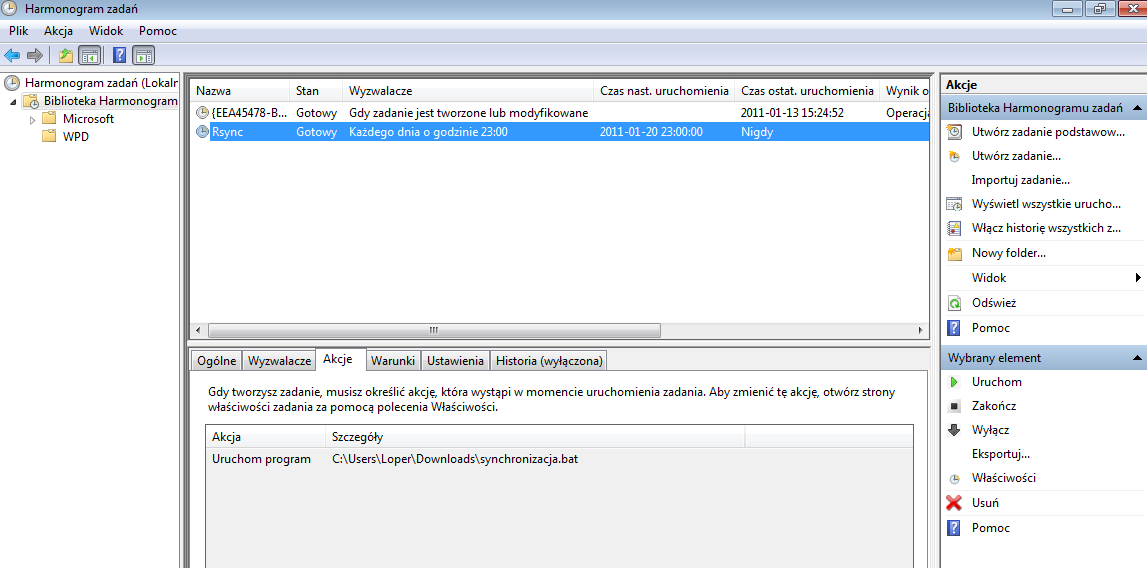
\includegraphics[width=0.8\textwidth]{../img/harmon.jpg}
	\caption{Harmonogram zadań na Windows 7}
	\label{harm}
\end{figure}

\end{enumerate}

Do każdego ze skryptów można dopisać na końcu linijkę \verb|PAUSE| - umożliwi ona wyświetlenie wyniku operacji - nie zamknie okna, jeśli wywołaliśmy skrypt bezpośrednio (to znaczy klikając na niego - nie z poziomu konsoli). W przypadku używania tych plików wsadowych w połączeniu z ,,Harmonogramem Zadań'', autostartem - kiedy jest automatycznie startowany, lepiej pominąć tą opcję (a nawet parametr \verb|verbose (-v)|), ponieważ w takiej sytuacji nie potrzebujemy okna z informacją. 

